\chapter{Complementos del SGDW}\label{chap:complemento-sgdw}  % MARK: Complemnetos del SGDW

\RED[inline]{Hay que revisar este párrafo}

En este anexo se presentan algunos detalles adicionales de la Sección~\ref{sec:sgdw} del Capítulo~\ref{chap:app-bar-wass}. A decir, algunos parámetros adicionales, e imágenes de las iteraciones del algoritmo.

\section{Parámetros Adicionales}\label{sec:compl-sgdw-params-adicional}  % MARK: - Parámetros adicionales

\RED[inline]{Hay que revisar esta sección}

En el Algoritmo~\ref{alg:sgdw-general} se menciona que este debe de recibir como entrada los parámetros $(\eta_k)_k \in [0, 1]^{\N}$ y $(S_k)_k \in \N_\ast^\N$. Sin embargo, no se menciona la manera de cálcular el baricentro en el paso 6. del algoritmo. En este trabajo, se utiliza una estimación del baricentro. Método el cuál también posee sus propios parámetros.

En los experimentos, se utiliza el método de Baricentros de Wasserstein Convolucionales Insesgados \cite{janati2020debiased}, implementada en la librería de POT \cite{flamary2021pot}. En particular, se utiliza la función \texttt{convolutional\_barycenter2d\_debiased} del módulo \texttt{ot.bregman} de POT con los siguientes parámetros:
\begin{itemize}
    \item \texttt{reg} fijado a $10^{-2}$.
    \item \texttt{numItermax} fijado a $10,000$.
    \item \texttt{stopThr} fijado a $10^{-3}$.
\end{itemize}

Estos parámetros han sido fijados de manera heurística, y no se ha realizado un estudio de sensibilidad de los mismos.

\section{Iteraciones del Algoritmo}\label{sec:compl-sgdw-iters}  % MARK: - Iteraciones del Algoritmo

\RED[inline]{Hay que revisar esta sección}

Adicional a los baricentros presentados en la Figura~\ref{fig:barycenters}, se han registrado las primeras y últimas iteraciones del cálculo de los baricentros. En partícular, se presenta la primera medida del muestreo de $\Gamma$, que corresponde a la línea 4. del  Algoritmo~\ref{alg:sgdw-general}; y seguidamente se presenta el paso del algoritmo, que corrresponde a la línea 6. de dicho algoritmo.

% MARK: - Empirica
\begin{figure}[htbp]
    \centering
    \begin{subfigure}[b]{0.95\textwidth}
        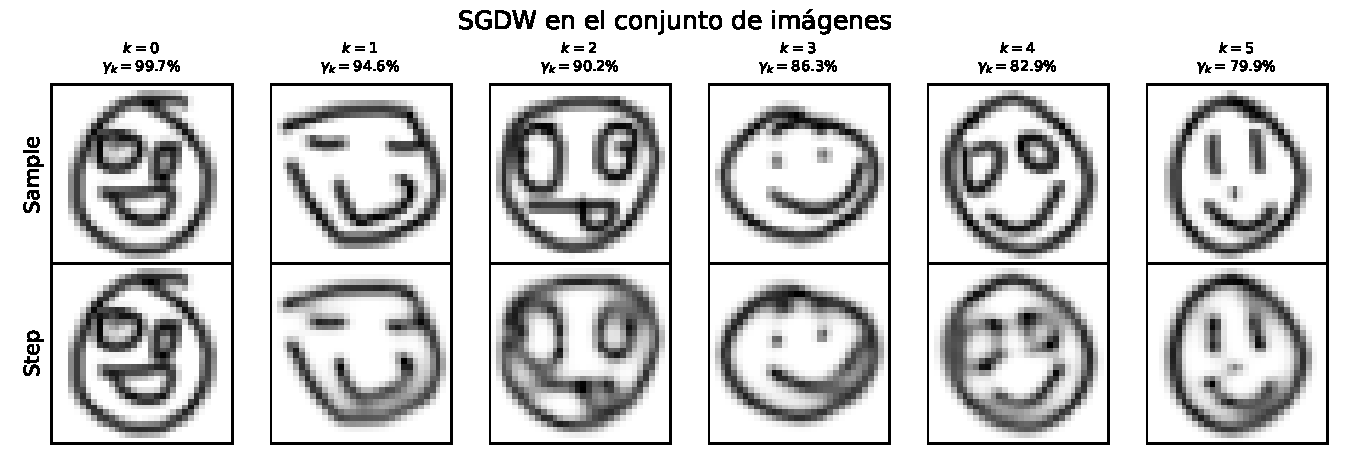
\includegraphics[width=\textwidth]{img/sgdw-iters/first-iters-DS.pdf}
        \caption{Primeras iteraciones.}
        \label{fig:first-iters-DS}
    \end{subfigure}
    \newline
    \begin{subfigure}[b]{0.95\textwidth}
        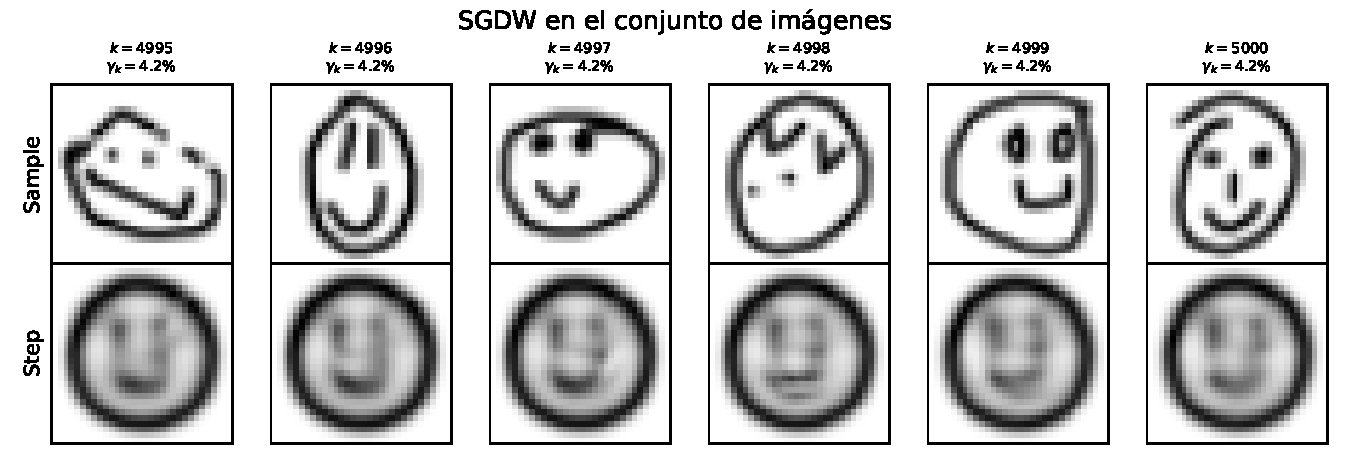
\includegraphics[width=\textwidth]{img/sgdw-iters/last-iters-DS.pdf}
        \caption{Últimas iteraciones.}
        \label{fig:last-iters-DS}
    \end{subfigure}
    \caption{Iteraciones del cálculo del baricentro de $\hat\Prob_X$.}
    \label{fig:iters-DS}
\end{figure}

% MARK: - GAN
\begin{figure}[htbp]
    \centering
    \begin{subfigure}[b]{0.95\textwidth}
        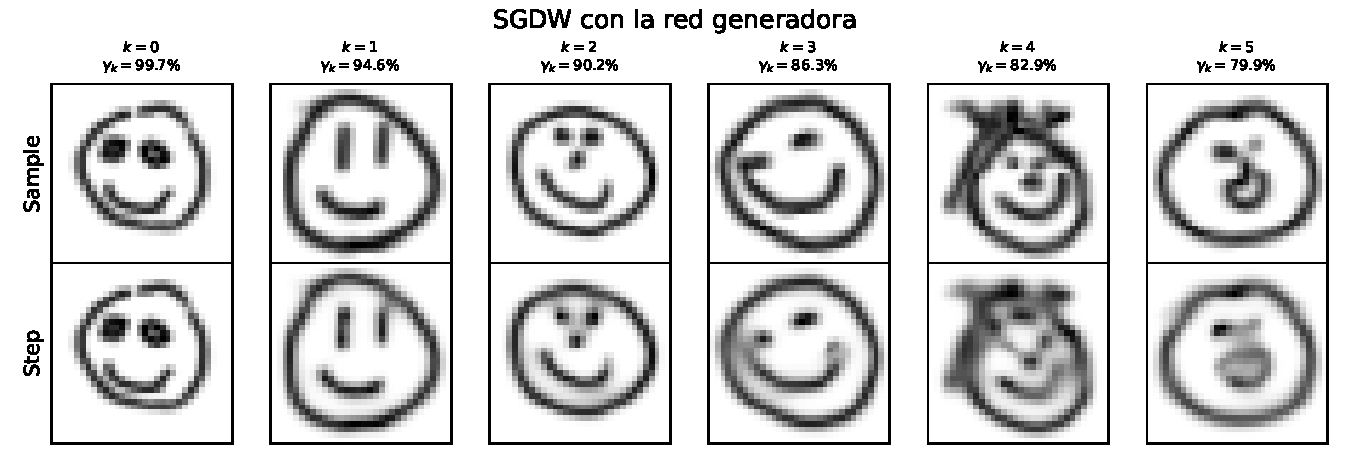
\includegraphics[width=\textwidth]{img/sgdw-iters/first-iters-GAN.pdf}
        \caption{Primeras iteraciones.}
        \label{fig:first-iters-GAN}
    \end{subfigure}
    \newline
    \begin{subfigure}[b]{0.95\textwidth}
        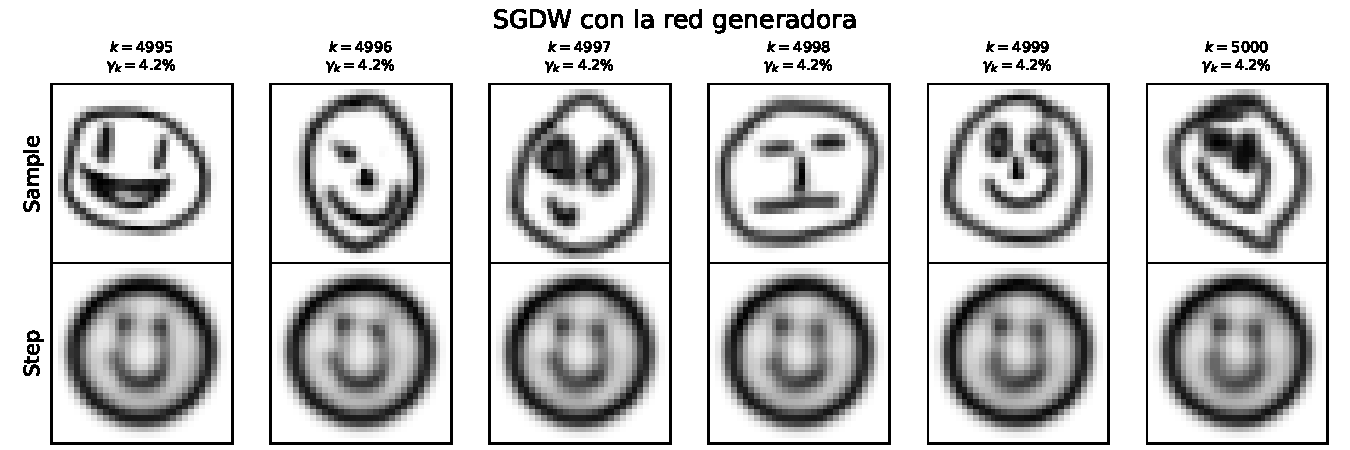
\includegraphics[width=\textwidth]{img/sgdw-iters/last-iters-GAN.pdf}
        \caption{Últimas iteraciones.}
        \label{fig:last-iters-GAN}
    \end{subfigure}
    \caption{Iteraciones del cálculo del baricentro de $\tilde\Prob_X$.}
    \label{fig:iters-GAN}
\end{figure}

% MARK: - Empirica Batched
\begin{figure}[htbp]
    \centering
    \begin{subfigure}[b]{0.95\textwidth}
        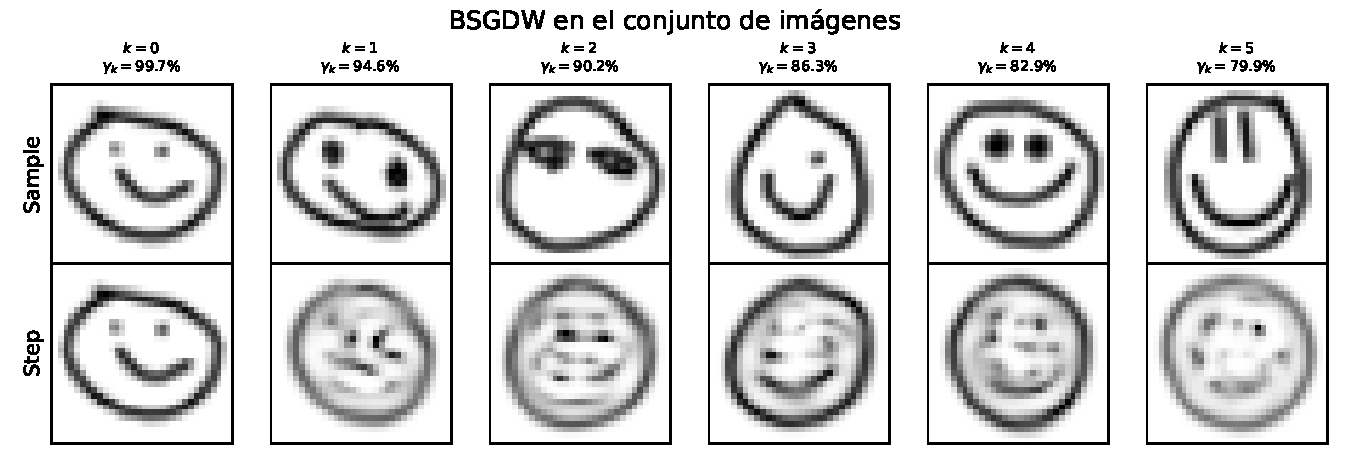
\includegraphics[width=\textwidth]{img/sgdw-iters/batch-first-iters-DS.pdf}
        \caption{Primeras iteraciones.}
        \label{fig:batch-first-iters-DS}
    \end{subfigure}
    \newline
    \begin{subfigure}[b]{0.95\textwidth}
        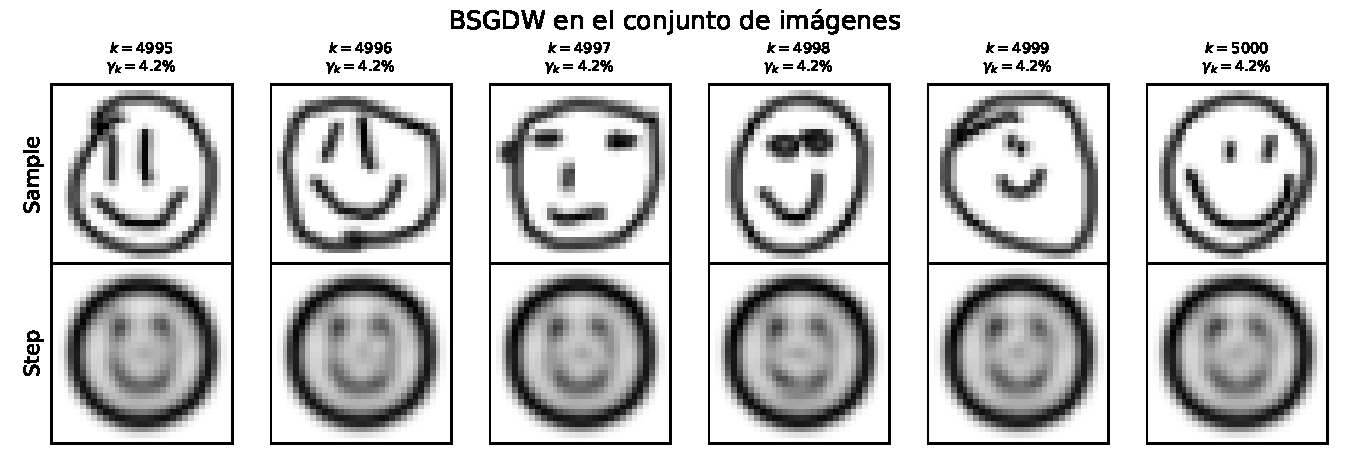
\includegraphics[width=\textwidth]{img/sgdw-iters/batch-last-iters-DS.pdf}
        \caption{Últimas iteraciones.}
        \label{fig:batch-last-iters-DS}
    \end{subfigure}
    \caption{Iteraciones del cálculo del baricentro de $\hat\Prob_X$ en su versión por lotes.}
    \label{fig:batch-iters-DS}
\end{figure}

% MARK: - GAN Batched
\begin{figure}[htbp]
    \centering
    \begin{subfigure}[b]{0.95\textwidth}
        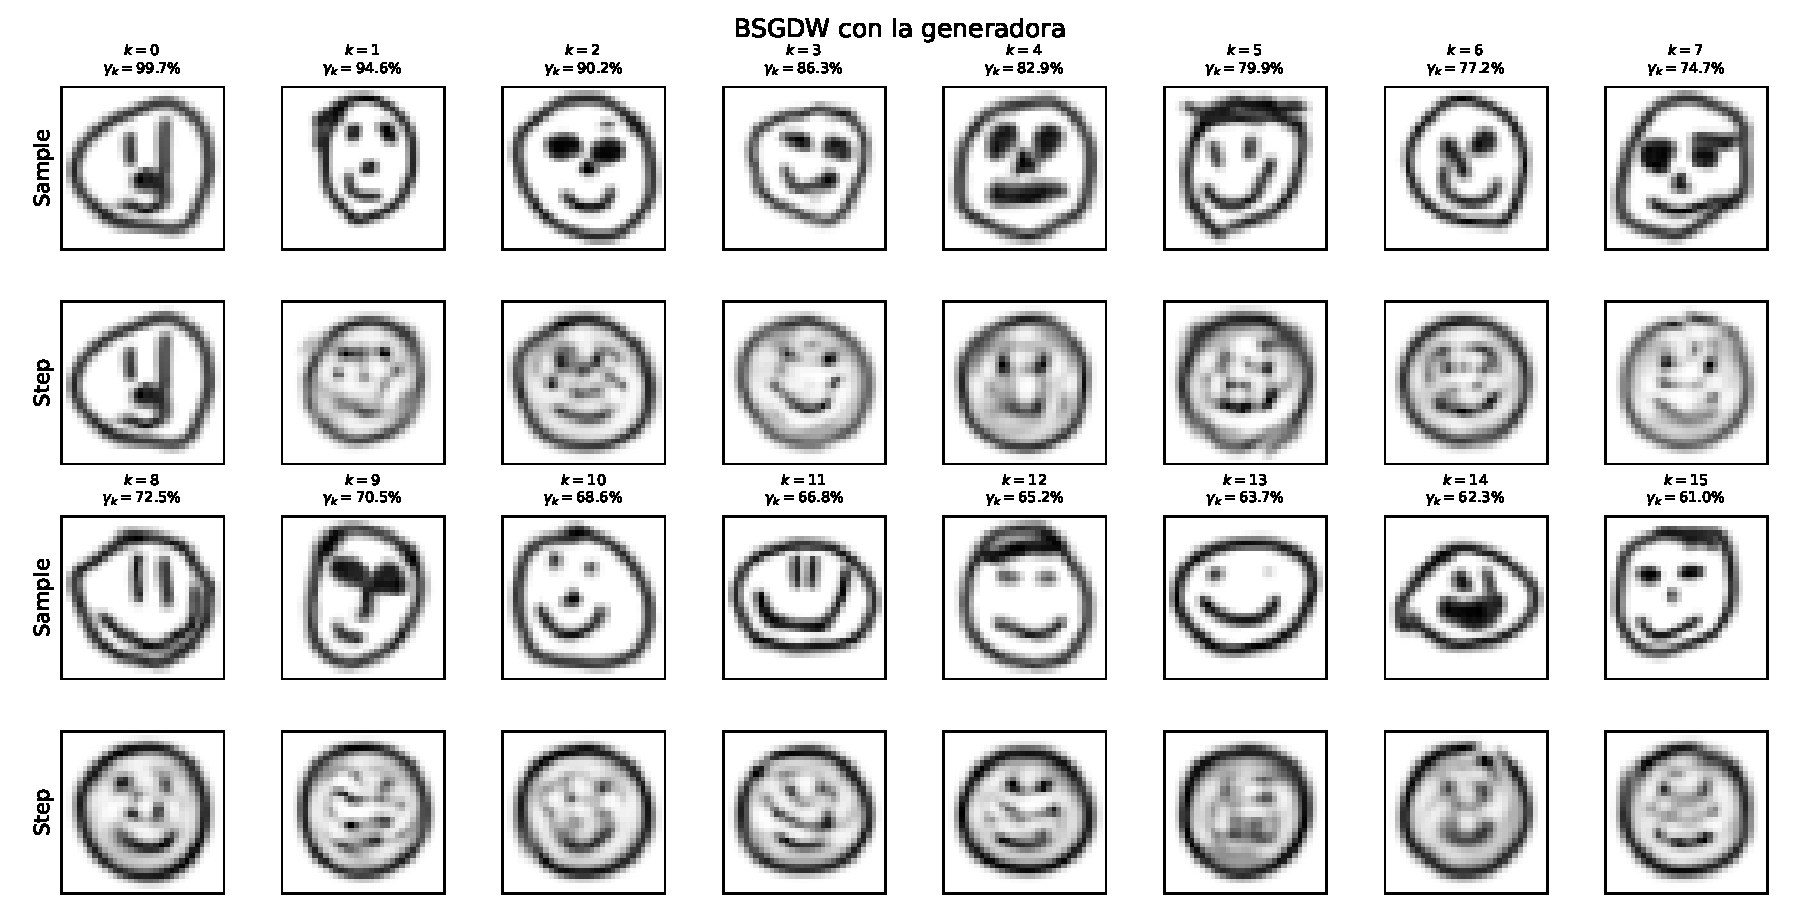
\includegraphics[width=\textwidth]{img/sgdw-iters/batch-first-iters-GAN.pdf}
        \caption{Primeras iteraciones.}
        \label{fig:batch-first-iters-GAN}
    \end{subfigure}
    \newline
    \begin{subfigure}[b]{0.95\textwidth}
        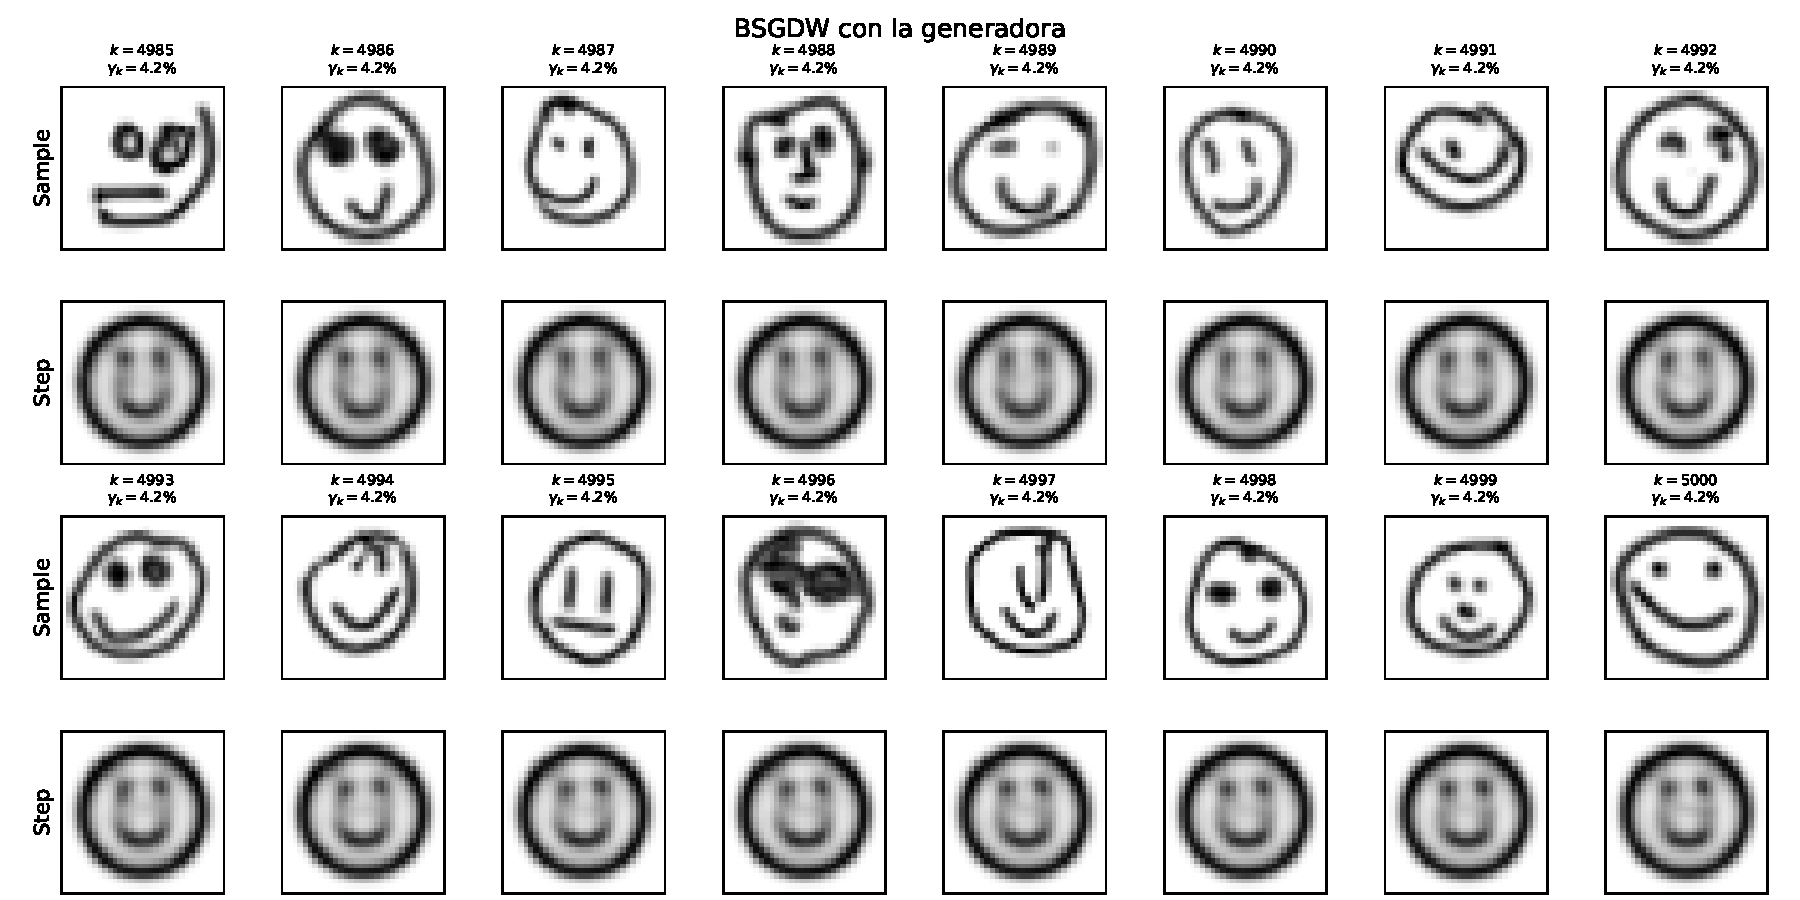
\includegraphics[width=\textwidth]{img/sgdw-iters/batch-last-iters-GAN.pdf}
        \caption{Últimas iteraciones.}
        \label{fig:batch-last-iters-GAN}
    \end{subfigure}
    \caption{Iteraciones del cálculo del baricentro de $\tilde\Prob_X$ en su versión por lotes.}
    \label{fig:batch-iters-GAN}
\end{figure}


